% 2011 年四川卷理科第 7 题：四个选项的函数图象（选项图）。
% 来源 PDF：普通高考/2011/2011四川理.pdf，SHA-256 116ce515679869425079ef4777505df3735ba4cba64847c9069b7d7acdb4fda4。
% 原页：第 1 页（A3 三栏）第 1 栏下部接第 2 栏上部，书页码 701。
% 重绘依据：题设 f 为 R 上奇函数，x>0 时 f(x)=(1/2)^x+1，故 f(0)=0，
%   x<0 时 f(x)=-(2^x+1)；f 在 R 上单射，反函数 g=f^{-1} 满足
%   x∈(1,2) 时 g(x)=log_{1/2}(x-1)，x∈(-2,-1) 时 g(x)=log_2(-x-1)，g(0)=0。
%   照原页：(A) 为 y=g(x)；(B) 为 y=f(x)；(C) 为 y=f(-x)；(D) 为 y=-g(x)。
%   端点空心圆、原点实心点、竖直渐近线位置均照原页，不按比例。
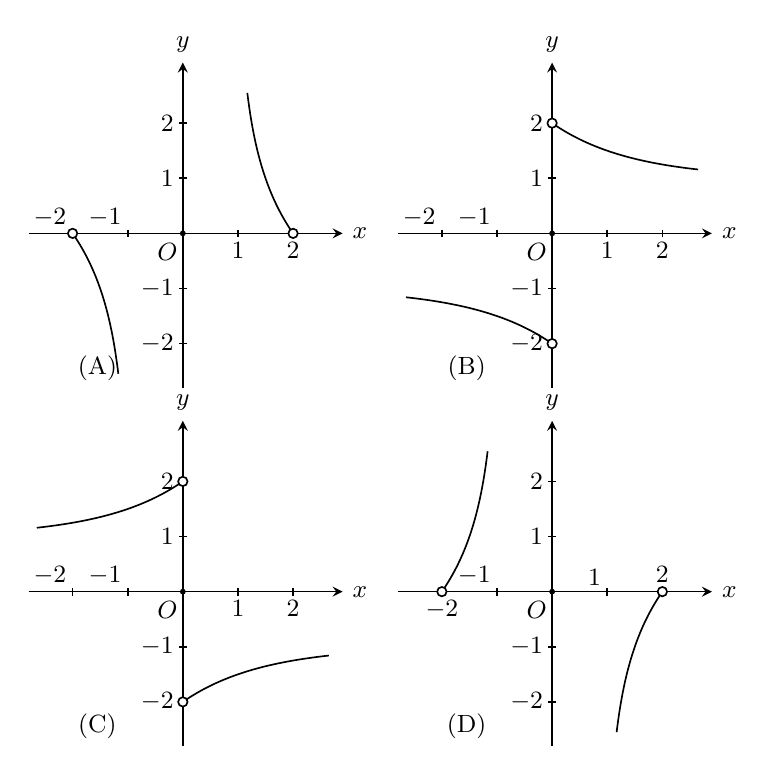
\begin{tikzpicture}[scale=0.70, >=stealth, semithick, font=\small,
  dec/.style={fill=white, draw=black}]

  % ================= (A) y = f^{-1}(x) =================
  \begin{scope}
    \draw[->] (-2.8,0) -- (2.9,0) node[right] {$x$};
    \draw[->] (0,-2.8) -- (0,3.1) node[above] {$y$};
    \foreach \t in {-2,-1,1,2} { \draw (\t,0.07) -- (\t,-0.07); }
    \foreach \t in {-2,-1,1,2} { \draw (0.07,\t) -- (-0.07,\t); }
    \node[above left, inner sep=2pt] at (-2,0) {$-2$};
    \node[above left, inner sep=2pt] at (-1,0) {$-1$};
    \node[below, inner sep=3pt] at (1,0) {$1$};
    \node[below, inner sep=3pt] at (2,0) {$2$};
    \node[left, inner sep=3pt] at (0,1) {$1$};
    \node[left, inner sep=3pt] at (0,2) {$2$};
    \node[left, inner sep=3pt] at (0,-1) {$-1$};
    \node[left, inner sep=3pt] at (0,-2) {$-2$};
    \node at (-0.28,-0.34) {$O$};
    \draw[domain=-1.96:-1.17, samples=70] plot (\x,{ln(-\x-1)/ln(2)});
    \draw[domain=1.17:1.96, samples=70] plot (\x,{-ln(\x-1)/ln(2)});
    \node[dec] at (-2,0) [circle, inner sep=0pt, minimum size=3.4pt] {};
    \node[dec] at (2,0)  [circle, inner sep=0pt, minimum size=3.4pt] {};
    \fill (0,0) circle (1.5pt);
    \node at (-1.55,-2.45) {(A)};
  \end{scope}

  % ================= (B) y = f(x) =================
  \begin{scope}[xshift=6.7cm]
    \draw[->] (-2.8,0) -- (2.9,0) node[right] {$x$};
    \draw[->] (0,-2.8) -- (0,3.1) node[above] {$y$};
    \foreach \t in {-2,-1,1,2} { \draw (\t,0.07) -- (\t,-0.07); }
    \foreach \t in {-2,-1,1,2} { \draw (0.07,\t) -- (-0.07,\t); }
    \node[above left, inner sep=2pt] at (-2,0) {$-2$};
    \node[above left, inner sep=2pt] at (-1,0) {$-1$};
    \node[below, inner sep=3pt] at (1,0) {$1$};
    \node[below, inner sep=3pt] at (2,0) {$2$};
    \node[left, inner sep=3pt] at (0,1) {$1$};
    \node[left, inner sep=3pt] at (0,2) {$2$};
    \node[left, inner sep=3pt] at (0,-1) {$-1$};
    \node[left, inner sep=3pt] at (0,-2) {$-2$};
    \node at (-0.28,-0.34) {$O$};
    \draw[domain=0.06:2.65, samples=70] plot (\x,{exp(-\x*ln(2))+1});
    \draw[domain=-2.65:-0.06, samples=70] plot (\x,{-exp(\x*ln(2))-1});
    \node[dec] at (0,2) [circle, inner sep=0pt, minimum size=3.4pt] {};
    \node[dec] at (0,-2) [circle, inner sep=0pt, minimum size=3.4pt] {};
    \fill (0,0) circle (1.5pt);
    \node at (-1.55,-2.45) {(B)};
  \end{scope}

  % ================= (C) y = f(-x) =================
  \begin{scope}[yshift=-6.5cm]
    \draw[->] (-2.8,0) -- (2.9,0) node[right] {$x$};
    \draw[->] (0,-2.8) -- (0,3.1) node[above] {$y$};
    \foreach \t in {-2,-1,1,2} { \draw (\t,0.07) -- (\t,-0.07); }
    \foreach \t in {-2,-1,1,2} { \draw (0.07,\t) -- (-0.07,\t); }
    \node[above left, inner sep=2pt] at (-2,0) {$-2$};
    \node[above left, inner sep=2pt] at (-1,0) {$-1$};
    \node[below, inner sep=3pt] at (1,0) {$1$};
    \node[below, inner sep=3pt] at (2,0) {$2$};
    \node[left, inner sep=3pt] at (0,1) {$1$};
    \node[left, inner sep=3pt] at (0,2) {$2$};
    \node[left, inner sep=3pt] at (0,-1) {$-1$};
    \node[left, inner sep=3pt] at (0,-2) {$-2$};
    \node at (-0.28,-0.34) {$O$};
    \draw[domain=-2.65:-0.06, samples=70] plot (\x,{exp(\x*ln(2))+1});
    \draw[domain=0.06:2.65, samples=70] plot (\x,{-exp(-\x*ln(2))-1});
    \node[dec] at (0,2) [circle, inner sep=0pt, minimum size=3.4pt] {};
    \node[dec] at (0,-2) [circle, inner sep=0pt, minimum size=3.4pt] {};
    \fill (0,0) circle (1.5pt);
    \node at (-1.55,-2.45) {(C)};
  \end{scope}

  % ================= (D) y = -f^{-1}(x) =================
  \begin{scope}[xshift=6.7cm, yshift=-6.5cm]
    \draw[->] (-2.8,0) -- (2.9,0) node[right] {$x$};
    \draw[->] (0,-2.8) -- (0,3.1) node[above] {$y$};
    \foreach \t in {-2,-1,1,2} { \draw (\t,0.07) -- (\t,-0.07); }
    \foreach \t in {-2,-1,1,2} { \draw (0.07,\t) -- (-0.07,\t); }
    \node[below, inner sep=3pt] at (-2,0) {$-2$};
    \node[above left, inner sep=2pt] at (-1,0) {$-1$};
    \node[above left, inner sep=2pt] at (1,0) {$1$};
    \node[above, inner sep=3pt] at (2,0) {$2$};
    \node[left, inner sep=3pt] at (0,1) {$1$};
    \node[left, inner sep=3pt] at (0,2) {$2$};
    \node[left, inner sep=3pt] at (0,-1) {$-1$};
    \node[left, inner sep=3pt] at (0,-2) {$-2$};
    \node at (-0.28,-0.34) {$O$};
    \draw[domain=-1.96:-1.17, samples=70] plot (\x,{-ln(-\x-1)/ln(2)});
    \draw[domain=1.17:1.96, samples=70] plot (\x,{ln(\x-1)/ln(2)});
    \node[dec] at (-2,0) [circle, inner sep=0pt, minimum size=3.4pt] {};
    \node[dec] at (2,0)  [circle, inner sep=0pt, minimum size=3.4pt] {};
    \fill (0,0) circle (1.5pt);
    \node at (-1.55,-2.45) {(D)};
  \end{scope}

\end{tikzpicture}
